\documentclass[border=12pt]{standalone}

\usepackage{tikz}
\usetikzlibrary{
  positioning,
  arrows.meta,
  fit,
  backgrounds
}

\begin{document}

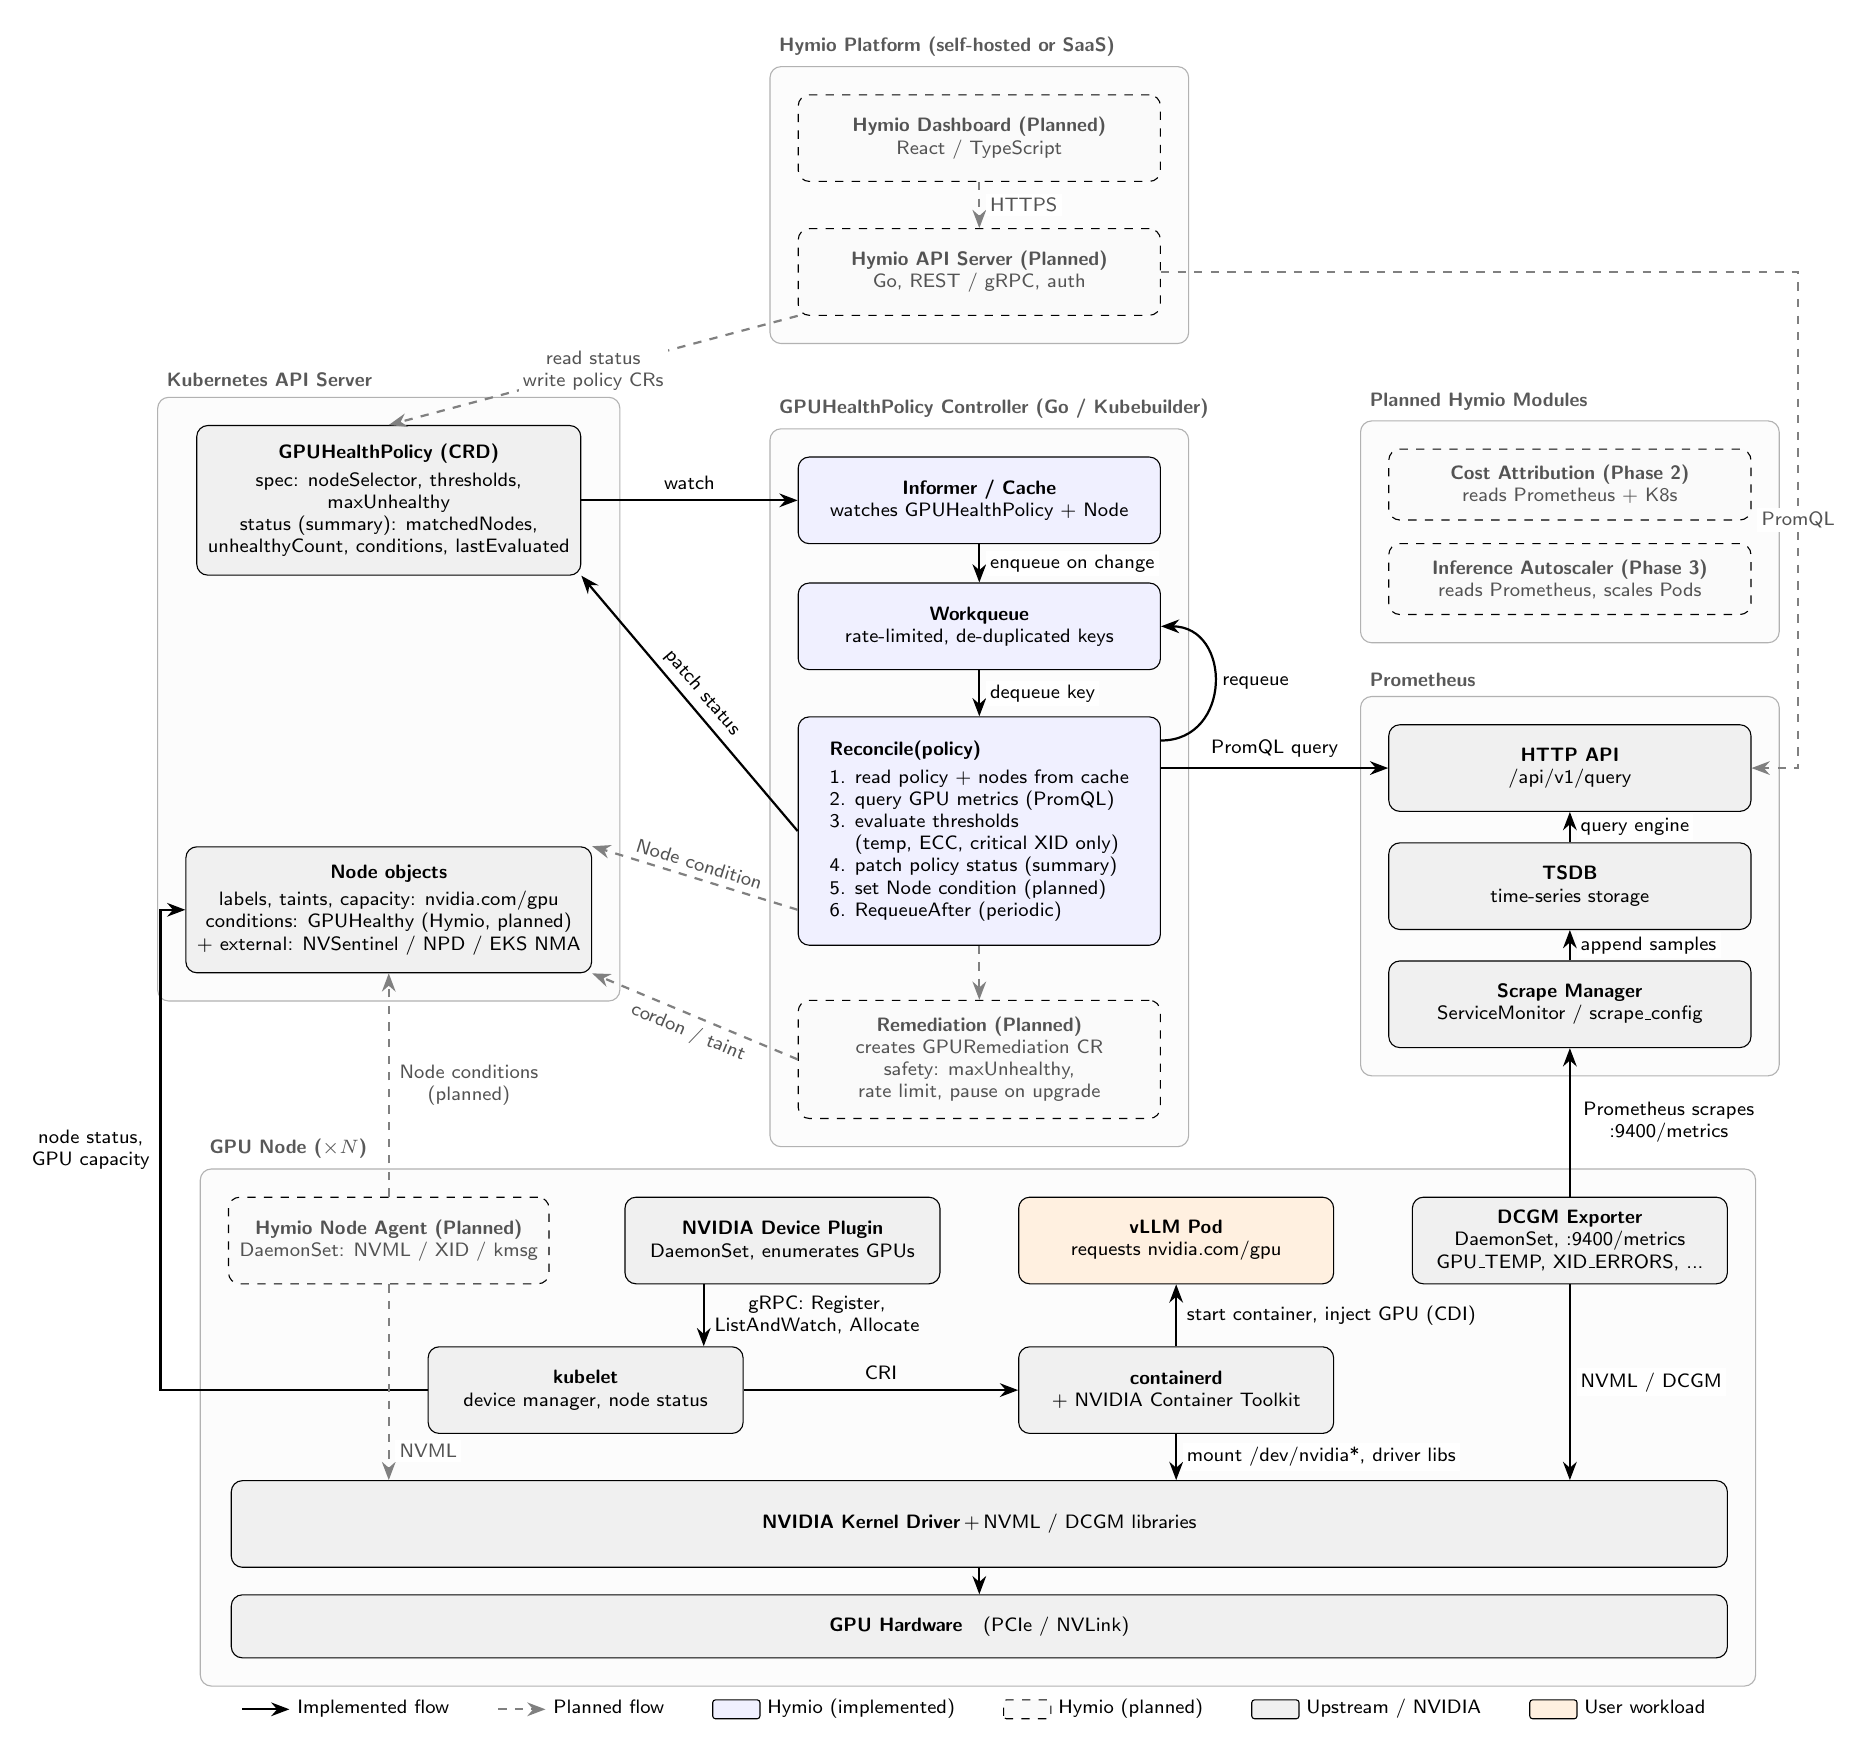
\begin{tikzpicture}[
  font=\sffamily\scriptsize,
  base/.style={
    draw,
    rounded corners,
    minimum width=4.6cm,
    minimum height=1.1cm,
    align=center,
    inner sep=4pt
  },
  hymio/.style={base, fill=blue!6},
  upstream/.style={base, fill=gray!12},
  workload/.style={base, fill=orange!12},
  planned/.style={base, dashed, fill=gray!4, text=gray!65!black},
  nodebox/.style={minimum width=4cm},
  arrow/.style={-{Stealth}, thick},
  parrow/.style={-{Stealth}, thick, dashed, gray},
  lbl/.style={fill=white, inner sep=1.5pt, align=center},
  plbl/.style={lbl, text=gray!65!black},
  group/.style={
    draw=gray!60,
    rounded corners,
    inner sep=10pt,
    fill=gray!2
  },
  grouplabel/.style={font=\sffamily\scriptsize\bfseries, text=gray!70!black}
]

% ================= Layer 1: Hymio platform (planned) =================
\node[planned] (dashboard) at (0, 0)
  {\textbf{Hymio Dashboard (Planned)}\\React / TypeScript};
\node[planned] (api) at (0, -1.7)
  {\textbf{Hymio API Server (Planned)}\\Go, REST / gRPC, auth};

% ================= Layer 2: Kubernetes API objects =================
\node[upstream, minimum height=1.9cm] (crd) at (-7.5, -4.6)
  {\textbf{GPUHealthPolicy (CRD)}\\[2pt]
   spec: nodeSelector, thresholds,\\maxUnhealthy\\
   status (summary): matchedNodes,\\unhealthyCount, conditions, lastEvaluated};
\node[upstream, minimum height=1.6cm] (nodes) at (-7.5, -9.8)
  {\textbf{Node objects}\\[2pt]
   labels, taints, capacity: nvidia.com/gpu\\
   conditions: GPUHealthy (Hymio, planned)\\
   + external: NVSentinel / NPD / EKS NMA};

% ================= Layer 2: Hymio controller =================
\node[hymio] (informer) at (0, -4.6)
  {\textbf{Informer / Cache}\\watches GPUHealthPolicy + Node};
\node[hymio] (wq) at (0, -6.2)
  {\textbf{Workqueue}\\rate-limited, de-duplicated keys};
\node[hymio, minimum height=2.9cm, align=left] (rec) at (0, -8.8)
  {\textbf{Reconcile(policy)}\\[2pt]
   1. read policy + nodes from cache\\
   2. query GPU metrics (PromQL)\\
   3. evaluate thresholds\\
   \phantom{3. }(temp, ECC, critical XID only)\\
   4. patch policy status (summary)\\
   5. set Node condition (planned)\\
   6. RequeueAfter (periodic)};
\node[planned, minimum height=1.5cm] (remed) at (0, -11.7)
  {\textbf{Remediation (Planned)}\\creates GPURemediation CR\\
   safety: maxUnhealthy,\\rate limit, pause on upgrade};

% ================= Layer 2: planned modules =================
\node[planned, minimum height=0.9cm] (cost) at (7.5, -4.4)
  {\textbf{Cost Attribution (Phase 2)}\\reads Prometheus + K8s};
\node[planned, minimum height=0.9cm] (scaler) at (7.5, -5.6)
  {\textbf{Inference Autoscaler (Phase 3)}\\reads Prometheus, scales Pods};

% ================= Layer 2: Prometheus =================
\node[upstream] (promapi) at (7.5, -8.0)
  {\textbf{HTTP API}\\/api/v1/query};
\node[upstream] (tsdb) at (7.5, -9.5)
  {\textbf{TSDB}\\time-series storage};
\node[upstream] (scrape) at (7.5, -11.0)
  {\textbf{Scrape Manager}\\ServiceMonitor / scrape\_config};

% ================= Layer 3: GPU node =================
\node[planned, nodebox] (agent) at (-7.5, -14.0)
  {\textbf{Hymio Node Agent (Planned)}\\DaemonSet: NVML / XID / kmsg};
\node[upstream, nodebox] (devplugin) at (-2.5, -14.0)
  {\textbf{NVIDIA Device Plugin}\\DaemonSet, enumerates GPUs};
\node[workload, nodebox] (vllm) at (2.5, -14.0)
  {\textbf{vLLM Pod}\\requests nvidia.com/gpu};
\node[upstream, nodebox] (dcgm) at (7.5, -14.0)
  {\textbf{DCGM Exporter}\\DaemonSet, :9400/metrics\\
   GPU\_TEMP, XID\_ERRORS, ...};

\node[upstream, nodebox] (kubelet) at (-5.0, -15.9)
  {\textbf{kubelet}\\device manager, node status};
\node[upstream, nodebox] (containerd) at (2.5, -15.9)
  {\textbf{containerd}\\+ NVIDIA Container Toolkit};

\node[upstream, minimum width=19cm] (driver) at (0, -17.6)
  {\textbf{NVIDIA Kernel Driver}\,+\,NVML / DCGM libraries};
\node[upstream, minimum width=19cm, minimum height=0.8cm] (hw) at (0, -18.9)
  {\textbf{GPU Hardware}\quad (PCIe / NVLink)};

% ================= Group frames =================
\begin{scope}[on background layer]
  \node[group, fit=(dashboard)(api),
        label={[grouplabel, anchor=south west]north west:Hymio Platform (self-hosted or SaaS)}] {};
  \node[group, fit=(crd)(nodes),
        label={[grouplabel, anchor=south west]north west:Kubernetes API Server}] {};
  \node[group, fit=(informer)(wq)(rec)(remed),
        label={[grouplabel, anchor=south west]north west:GPUHealthPolicy Controller (Go / Kubebuilder)}] {};
  \node[group, fit=(cost)(scaler),
        label={[grouplabel, anchor=south west]north west:Planned Hymio Modules}] {};
  \node[group, fit=(promapi)(tsdb)(scrape),
        label={[grouplabel, anchor=south west]north west:Prometheus}] {};
  \node[group, fit=(agent)(devplugin)(vllm)(dcgm)(kubelet)(containerd)(driver)(hw),
        label={[grouplabel, anchor=south west]north west:GPU Node ($\times N$)}] {};
\end{scope}

% ================= Arrows: platform (planned) =================
\draw[parrow] (dashboard) -- node[plbl, right=2pt] {HTTPS} (api);
\draw[parrow] (api.south west) -- node[plbl, pos=0.5] {read status\\write policy CRs} (crd.north);
\draw[parrow] (api.east) -- (10.4, -1.7) |- node[plbl, pos=0.25] {PromQL} (promapi.east);

% ================= Arrows: controller loop =================
\draw[arrow] (crd.east |- informer.west) -- node[lbl, above=2pt, fill=none] {watch} (informer.west);
\draw[arrow] (informer) -- node[lbl, right=2pt] {enqueue on change} (wq);
\draw[arrow] (wq) -- node[lbl, right=2pt] {dequeue key} (rec.north);
\draw[arrow] ([yshift=1.15cm]rec.east) to[out=0, in=0, looseness=1.6]
  node[lbl, right=1pt] {requeue} (wq.east);
\draw[arrow] (rec.east |- promapi.west) -- node[lbl, above=2pt, fill=none] {PromQL query} (promapi.west);
\draw[arrow] (rec.west) -- node[lbl, sloped, above=1pt, fill=none] {patch status} (crd.south east);
\draw[parrow] (remed.west) -- node[plbl, sloped, below=1pt, fill=none] {cordon / taint} (nodes.south east);
\draw[parrow] ([yshift=-1.0cm]rec.west) -- node[plbl, sloped, above=1pt, fill=none] {Node condition} (nodes.north east);
\draw[parrow] (rec.south) -- (remed.north);

% ================= Arrows: Prometheus internals =================
\draw[arrow] (scrape) -- node[lbl, right=2pt] {append samples} (tsdb);
\draw[arrow] (tsdb) -- node[lbl, right=2pt] {query engine} (promapi);
\draw[arrow] (dcgm.north) -- node[lbl, right=3pt] {Prometheus scrapes\\:9400/metrics} (scrape.south);

% ================= Arrows: GPU node =================
\draw[arrow] ([xshift=-1cm]devplugin.south) -- node[lbl, right=2pt, fill=none] {gRPC: Register,\\ListAndWatch, Allocate}
  ([xshift=-1cm]devplugin.south |- kubelet.north);
\draw[arrow] (kubelet.east) -- node[lbl, above=2pt, fill=none] {CRI} (containerd.west);
\draw[arrow] (containerd.north) -- node[lbl, right=2pt, fill=none] {start container, inject GPU (CDI)} (vllm.south);
\draw[arrow] (kubelet.west) -- (-10.4, -15.9) |- node[lbl, pos=0.25, left=2pt] {node status,\\GPU capacity} (nodes.west);
\draw[parrow] (agent.north) -- node[plbl, right=2pt] {Node conditions\\(planned)} (nodes.south -| agent.north);

\draw[arrow] (containerd.south) -- node[lbl, right=2pt] {mount /dev/nvidia*, driver libs} (containerd.south |- driver.north);
\draw[arrow] (dcgm.south) -- node[lbl, right=2pt] {NVML / DCGM} (dcgm.south |- driver.north);
\draw[parrow] (agent.south) -- node[plbl, pos=0.85, right=2pt] {NVML} (agent.south |- driver.north);
\draw[arrow] (driver) -- (hw);

% ================= Legend =================
\node[anchor=north west, align=left] at (-9.5, -19.7) {%
  \tikz[baseline=-0.5ex]{\draw[thick,-{Stealth}] (0,0)--(0.6,0);}~Implemented flow \qquad
  \tikz[baseline=-0.5ex]{\draw[thick,dashed,gray,-{Stealth}] (0,0)--(0.6,0);}~Planned flow \qquad
  \tikz[baseline=-0.5ex]{\draw[rounded corners=1pt,fill=blue!6] (0,-0.12) rectangle (0.6,0.12);}~Hymio (implemented) \qquad
  \tikz[baseline=-0.5ex]{\draw[dashed,rounded corners=1pt,fill=gray!4] (0,-0.12) rectangle (0.6,0.12);}~Hymio (planned) \qquad
  \tikz[baseline=-0.5ex]{\draw[rounded corners=1pt,fill=gray!12] (0,-0.12) rectangle (0.6,0.12);}~Upstream / NVIDIA \qquad
  \tikz[baseline=-0.5ex]{\draw[rounded corners=1pt,fill=orange!12] (0,-0.12) rectangle (0.6,0.12);}~User workload
};

\end{tikzpicture}

\end{document}